\documentclass{beamer}  %% オプションは環境や利用するプログラムに
%\documentclass[dvips,cjk]{beamer}   %% よって変える
\usepackage{luatexja}

%\AtBeginDvi{\special{pdf:tounicode 90ms-RKSJ-UCS2}} %% しおりが文字化けしないmように
\AtBeginDvi{\special{pdf:tounicode EUC-UCS2}}


%\setbeamertemplate{navigation symbols}{} %% 右下のアイコンを消す

\usetheme{CambridgeUS}         %% theme の選択
%\usetheme{Boadilla}           %% Beamer のディレクトリの中の
%\usetheme{Madrid}             %% beamerthemeCambridgeUS.sty を指定
%\usetheme{Antibes}            %% 色々と試してみるといいだろう
%\usetheme{Montpellier}        %% サンプルが beamer\doc に色々とある。
%\usetheme{Berkeley}
%\usetheme{Goettingen}
%\usetheme{Singapore}
%\usetheme{Szeged}

%\usecolortheme{rose}          %% colortheme を選ぶと色使いが変わる
%\usecolortheme{albatross}

%\useoutertheme{shadow}                 %% 箱に影をつける
%\usefonttheme{professionalfonts}       %% 数式の文字を通常の LaTeX と同じにする

\setbeamercovered{transparent}         %% 消えている文字をうっすらと表示する

\setbeamertemplate{theorems}[numbered]  %% 定理に番号をつける
\newtheorem{thm}{Theorem}[section]
\newtheorem{proposition}[thm]{Proposition}
\theoremstyle{example}
\newtheorem{exam}[thm]{Example}
\newtheorem{remark}[thm]{Remark}
\newtheorem{question}[thm]{Question}
\newtheorem{prob}[thm]{Problem}

\AtBeginSection[]
{
  \begin{frame}<beamer>
    \frametitle{Outline}
    \tableofcontents[currentsection,currentsubsection]
  \end{frame}
}


\begin{document}
\title[Beamer]{Beamer の使い方} 
\author[Nushio]{村主崇行}            %% ここに書かれた情報は色々なところに使われるので
\institute[Kyoto Univ.]{京都大学}   %% なるべく設定した方が良い
\date{Jan 17, 2014}

\begin{frame}                  %% \begin{frame}..\end{frame} で 1 枚のスライド
\titlepage                     %% タイトルページ
\end{frame}

\begin{frame}                  %% 目次 (必要なければ省略)
\tableofcontents
\end{frame}

\section{Mooreの法則の歴史}          
\subsection{原典}
\begin{frame}\frametitle{\insertsubsection}
\begin{quote}
The complexity for minimum component costs has increased at a rate of roughly {\bf a factor of two per year}. Certainly over the short term this rate can be expected to continue, if not to increase. Over the longer term, the rate of increase is a bit more uncertain, although there is no reason to believe it will not remain nearly constant for at least 10 years. That means by 1975, {\bf the number of components per integrated circuit} for minimum cost will be 65,000. I believe that such a large circuit can be built on a single wafer.
\end{quote}
\begin{flushright}
--- Gordon Moore, "Cramming more components onto integrated circuits", Electronics Magazine 19 April {\bf 1965}
\end{flushright}

\end{frame}

\begin{frame}\frametitle{原典の価値}
\small

In April 2005, Intel offered US \$10,000 to purchase a copy of the original Electronics Magazine issue in which Moore's article appeared.  David Clark, an engineer living in the United Kingdom
 had found the prized magazine under his floorboards
 and offer it to Intel.

\pause
David Clark had kept copies of the magazine for years, despite pleas from his wife to throw them away.

\pause
"I am really pleased about it because I studied physics and have always had interest in electronics. I could see the next 30 years were going to go like Moore's Law said, so I decided to go into electronics."

\begin{center}
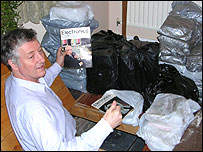
\includegraphics[height=4cm]{moores_magfound.jpg}
\end{center}

\end{frame}



\subsection{3年で4倍の初出}
\begin{frame}\frametitle{3年で4倍の初出}
\begin{quote}
 "Moore also affirmed he never said transistor count would double every 18 months, as is commonly said. Initially, he said transistors on a chip would double every year. He then recalibrated it to every two years in 1975. David House, an Intel executive at the time, noted that the changes would cause computer performance to double every 18 months."
\end{quote}
\begin{flushright}
--- Michael Kanellos, 2011 
\end{flushright}
\end{frame}


\begin{frame}
\begin{quote}
His prediction has proven to be accurate, in part because the law is now used in the semiconductor industry to guide long-term planning and to set targets for research and development.
\end{quote}

\begin{flushright}
--- Disco and Meulen (1998).
\end{flushright}
\end{frame}


\subsection{Mooreの法則・派生版}
\begin{frame}
\begin{itemize}\frametitle{\insertsubsection}
\item {\bf Transistor per integrated circuit} .
\item {\bf Computation speed} of a single chip.
\item {\bf Computation speed} of the world's fastest supercomputer .
\item {\bf Hard disk capacity per cost} roughly doubles in 18 months.
\item {\bf Network cable capacity} doubles every nine month.
\item {\bf Pixel per dollar} of a digital camera.
\item The great Moore's law compensator: {\bf Computation resource per given task} of Microsoft Office.

\end{itemize} 
\end{frame}

\section{Mooreの法則再確認 2014}             %% セクション名

\subsection{周波数} 
\begin{frame}\frametitle{\insertsubsection}
\begin{center}
\includegraphics[angle=270,width=7cm]{year_freq.eps}
\end{center}
\pause
\begin{itemize}
\item '00年代前半にサチった。\pause
\item 「Free lunch is over」\pause「失われた10年」
\end{itemize}
\end{frame}


\subsection{命令発行速度}       
\begin{frame}\frametitle{\insertsubsection}
\begin{center}
\includegraphics[angle=270,width=7cm]{year_mips.eps}
\end{center}
\pause
\begin{itemize}
\item MIPS = 1秒に100万命令発行できる能力 (Mega Instructions Per Second) \pause
\item スレッド数(含HT)×周波数 \pause 
\item これも2010年ころには伸びに翳りが。
\end{itemize}
\end{frame}

\subsection{ピーク浮動小数点演算性能}          
\begin{frame}\frametitle{\insertsubsection}
\begin{center}
\includegraphics[angle=270,width=7cm]{year_flops.eps}
\end{center}
\begin{itemize}
\item CPUはやはり脱落気味?\pause
\item GPUは「Supermoore」と言って宣伝していたが…
\end{itemize}
\end{frame}

\subsection{TOP500}          
\begin{frame}\frametitle{\insertsubsection}
\begin{center}
\includegraphics[width=7cm,angle=270]{year_top500.eps}
\end{center}
\end{frame}


\end{document}

